<<<<<<< HEAD
In our scenario occupants enter and exit the room constantly, typically within seconds or minutes of each other, it is somewhat difficult to find the immediate use of predicting an occupant's future actions. However, our partner team from Kenya expressed a need for such a system because they have had issues with thefts. Incorporating such a feature to their surveillance systems could warn a guard whenever suspicious activity might occur. A suspicious activity could involve a person moving too close to a given exit - possibly leading to a restricted area. In order to calculate a somewhat reliable prediction, we need to capture and store data about the behavior of previous occupants. When the data set grows, the prediction gradually becomes more precise. In order to satisfy the prediction requirement, various existing solutions have been considered, namely the \emph{k-nearest neighbors algorithm} and an existing prediction model, the hidden Markov model.
=======
In our scenario occupants enter and exit the room constantly, typically within seconds or minutes of each other, it is somewhat difficult to find the immediate use of predicting an occupant's future actions. However, our partner team from Kenya expressed a need for such a system because they have had issues with thefts. Incorporating such a feature to their surveillance systems could warn a guard whenever suspicious activity might occur. A suspicious activity could involve a person moving too close to a given exit - possibly leading to a restricted area. In order to calculate a somewhat reliable prediction, we need to capture and store data about the behavior of previous occupants. When the data set grows, the prediction gradually becomes more precise. In order to satisfy the prediction requirement, various existing solutions have been considered, namely the \emph{k-nearest neighbors algorithm} and an existing prediction model, the hidden Markov model. 
>>>>>>> bec694a634c69c49faaaf44ccf3c8b7419794ec6

The former assigns a given object to a group depending on the \emph{k} nearest objects. To apply this to our scenario we had to do some creative thinking. Imagine storing the paths of each occupant in the past ultimately leading to an exit. We could create a group for each exit. Each point along a path would be put in the group matching the exit the path lead to. Now, given any position, we could analyze the \emph{k} closest neighboring previous points not part of the same path. Since each point is a part of a different path, the predicted exit would be where the majority of these paths lead to.
\begin{figure}[htb]
\centering
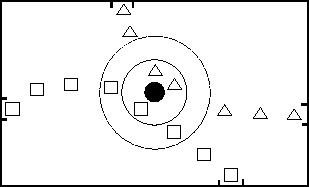
\includegraphics{prediction_figures/knn_room}
\caption{An illustration of the \emph{k-nearest neighbors algorithm}.}
\label{fig:knn}
\end{figure}
Figure~\ref{fig:knn} depicts an example where the center dot is the current position and the squares and triangles are previous occupant positions who chose separate exits. A \emph{k} of 3 selects the 3 nearest objects as illustrated by the inner circle. This would result in the occupant residing at the black dot is predicted to choose the same exit as the occupants previously positioned at the triangle positions. A \emph{k} of 5 selects the 5 nearest objects instead as illustrated by the circle with the dashed line. This yields a different output where the occupant is predicted to choose the same exit as the occupants represented by the squares. The approach has proven to be inefficient on larger data sets~\cite{bhatia}, which can be averted by performing clever data reduction. This, however, deemed the approach out of the scope of this project.
\begin{figure}[htb]
\centering
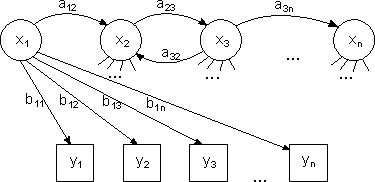
\includegraphics{prediction_figures/markov}
\caption{An illustration of a hidden Markov model.}
\label{fig:markov}
\end{figure}

<<<<<<< HEAD
Figure \ref{fig:markov} depicts the different parameters a hidden Markov model works with. Each \(x\) is a state and each \(y\) is a possible observation, where \(a\) is a state transition probability and \(b\) is an output probability. To map this to our scenario we need to define what exactly a state and an observation is and how to calculate the different probabilities. Since the ultimate goal is to predict what exit an occupant is going to take, a possible observation could be that an occupant exits a room at a given location. A state could represent an occupant residing in a given area of the room where a transition to another area would have a state transition probability \(a\). Given an occupant residing in a specific area of the room, say state \(x_2\), \(b_{2-2}\) is the probability that the occupant will choose the exit in observation \(y_2\). Typically, the initialization phase is as follows; random probability values are assigned to \(a\) and \(b\) (NEEDS CORRECTION: maybe a ref to jahmm or something else(??)). Gradually, these values are updated through observed actions of occupants. Over time, the probabilities will come to reflect how the average occupant is moving given a current location, resulting in more accurate predictions - this process is commonly referred to as training. Without training the probabilities are not based on anything, resulting in highly inaccurate predictions. The accuracy of the predictions grow with the size of the training set.
=======
Figure \ref{fig:markov} depicts the different parameters a hidden Markov model works with. Each \(x\) is a state and each \(y\) is a possible observation, where \(a\) is a state transition probability and \(b\) is an output probability. To map this to our scenario we need to define what exactly a state and an observation is and how to calculate the different probabilities. Since the ultimate goal is to predict what exit an occupant is going to take, a possible observation could be that an occupant exits a room at a given location. A state could represent an occupant residing in a given area of the room where a transition to another area would have a state transition probability \(a\). Given an occupant residing in a specific area of the room, say state \(x_2\), \(b_{2-2}\) is the probability that the occupant will choose the exit in observation \(y_2\). Typically, the initialization phase is as follows; random probability values are assigned to \(a\) and \(b\) (NEEDS CORRECTION: maybe a ref to jahmm or something else(??)). Gradually, these values are updated through observed actions of occupants. Over time, the probabilities will come to reflect how the average occupant is moving given a current location, resulting in more accurate predictions - this process is commonly referred to as training. Without training the probabilities are not based on anything, resulting in highly inaccurate predictions. The accuracy of the predictions grow with the size of the training set. 
>>>>>>> bec694a634c69c49faaaf44ccf3c8b7419794ec6

However, imagine a scenario where an even number of occupants move from one exit to another in both directions, evenly split. At any location along the path the probabilities to each exit remain equal, since equally many previous occupants have taken each exit given the current location. As a design decision we deem it less likely that an occupant will suddenly switch direction to the opposite. Thus, depending on the direction of the occupant the probability to one exit should be higher than the other. So in an attempt to make the predictions more accurate in cases like this, we wanted to establish several rule sets about general occupant movement behavior and integrate those into the calculations. Thus, we chose to design our own prediction model, heavily inspired by the hidden Markov model, since the original interpretation of states and probabilities as depicted in figure \ref{fig:markov} is maintained. The custom model is explained in detail in Section~\ref{ssub:designcustomprediction}. 